\documentclass[12pt, letterpaper]{article}
\usepackage[utf8]{inputenc}
\usepackage{amsmath}
\usepackage{changepage}% http://ctan.org/pkg/changepage
\usepackage{titlesec} 
\usepackage{commath}
\usepackage{placeins}
\usepackage{caption}
\newcommand\tab[1][1cm]{\hspace*{#1}}
\titleformat{\subsection}[runin]{}{}{}{}[]
\usepackage{graphicx}


\title{CS M148 Homework 4}
\author{Hanna Co}
\date{Due: March 7, 2022}

\begin{document}
\maketitle
\newpage
\section{Interpretation of Coefficients in Linear Regression}
\subsection*{a)} Our model is $Y = \beta_0 + \beta_1X_1 + \beta_2X_2 + \beta_3X_1X_2$, where $Y$ is our prediction of how much a person's cholesterol will be lowered. $X_1$ represents drug usage, where $X_1=0$ indicates no drug, and $X_1=1$ indicates drug usage. Similarly, $X_2$ represents the individual's gender, where $X_2=0$ indicates that the individual is female, and $X_2=1$ indicates that the individual is male.

\subsection*{b)} $\beta_0$ is the average lowering of cholesterol when $X_1=X_2=0$ (female, no drug). $\beta_1$  is the average lowering of cholesterol for both genders when the drug is used, and $\beta_2$ is the average difference in cholesterol between men and women. $\beta_3$ is the average difference between the lowering of cholesterol in men who take the drug compared to women who don't take the drug.

\subsection*{c)} We can determine significance by using a t-test. We use our model to fit $n$ datasets, and generate means and standard deviation for $\beta_2$. We then calculate the t-test, and use p-values to determine significance. For example, if we have a threshold of 0.05, if we get a p-value less than 0.05 then we reject the hypothesis that the effect of the drug was significantly different in men compared to women.

\newpage
\section{ Interpretation of Coefficient in Logistic Regression}
\subsection*{a)}
(i) On average, someone who did not receive treatment and doesn't prefer A is $e^{3.135}$ times more likely to prefer A the second time they're asked.\\
(ii) $e^{3.135}$\\
(iii) yes

\subsection*{b)} (i) On average, someone who received the treatment is $e^{2.309}$ times less liekly to prefer A the second time they're asked.\\
(ii) $e^{3.135-2.309}$\\
(iii) A is far less popular among those who received the treatment.

\subsection*{c)} (i) One average, someone who preferred A initially is $e^{5.15}$ times less likely to prefer A the second time they're asked.\\
(ii) $e^{5.15}$\\
(iii) This implies that the treatment increases the odds of someone preferring B to A, if they previously preferred A.

\subsection*{d)} (i) On average, a one unit increase in Treatment x PreferA will result in a $e^{2.85}$ greater change of an individual preferring A the second time they're asked.\\
(ii) $e^{2.85}$


\newpage
\section{Decision Tree }
\subsection*{1.} We calculate the Gini Index for each of the features.\\\\
Chest Pain: $1-(\frac{3}{3}^2+\frac{0}{3}^2) = 0$\\
No Chest Pain: $1-(\frac{1}{3}^2+\frac{2}{3}^2) = 0.44$\\
Gini (Chest Pain): $\frac{3}{6}*0 + \frac{3}{6}*0.44 = 0.222$\\\\
Male: $1-(\frac{2}{4}^2+\frac{2}{4}^2) = 0.5$\\
Not Male: $1-(\frac{2}{2}^2+\frac{0}{2}^2) = 0$\\
Gini (Male): $\frac{4}{6}*0.5 + \frac{2}{6}*0 = 0.333$\\\\
Smokes: $1-(\frac{3}{4}^2+\frac{1}{4}^2) = 0.375$\\
Doesn't Smoke: $1-(\frac{1}{2}^2+\frac{1}{2}^2) = 0.5$\\
Gini (Smoke): $\frac{4}{6}*0.375 + \frac{2}{6}*0.5 = 0.417$\\\\
Exercises: $1-(\frac{2}{4}^2+\frac{2}{4}^2) = 0.5$\\
Doesn't Exercise: $1-(\frac{2}{2}^2+\frac{0}{2}^2) = 0$\\
Gini (Exercises): $\frac{4}{6}*0.5 + \frac{2}{6}*0 = 0.333$\\\\
\\
\begin{tabular}{ |c|c| } 
 \hline
 \textbf{Feature} & \textbf{Gini} \\ 
\hline
Chest Pain & 0.222 \\ 
\hline
Male & 0.333 \\ 
\hline
Smokes & 0.417 \\ 
 \hline
Exercises & 0.333 \\ 
 \hline
\end{tabular}\\\\
\\
Chest Pain has the lowest Gini Index, so we split on that feature.\\
\begin{figure}[h!]
  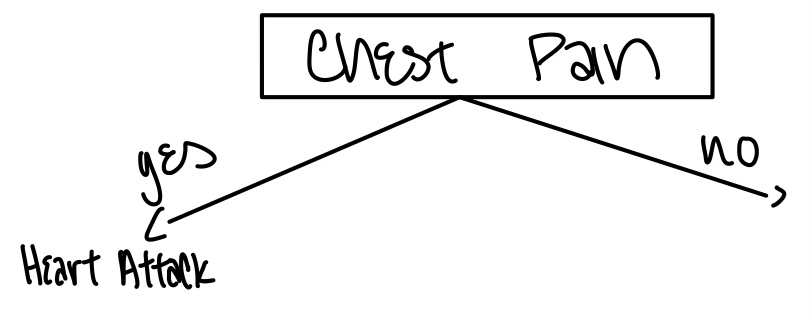
\includegraphics[scale=0.3]{./images/3.1_one}
\end{figure} \\
We calculate Gini Index Again to determine what features to split on.\\\\
Male: $1-(\frac{0}{2}^2+\frac{2}{2}^2) = 0$\\
Not Male: $1-(\frac{1}{1}^2+\frac{0}{1}^2) = 0$\\
Gini (Male): $\frac{2}{3}*0 + \frac{1}{3}*0 = 0$\\\\
Smokes: $1-(\frac{1}{2}^2+\frac{1}{2}^2) = 0.5$\\
Doesn't Smoke: $1-(\frac{0}{1}^2+\frac{1}{1}^2) = 0$\\
Gini (Smoke): $\frac{2}{3}*0.5 + \frac{1}{3}*0 = 0.333$\\\\
Exercises: $1-(\frac{0}{2}^2+\frac{2}{2}^2) = 0$\\
Doesn't Exercise: $1-(\frac{1}{1}^2+\frac{0}{1}^2) = 0$\\
Gini (Exercises): $\frac{2}{3}*0 + \frac{1}{3}*0 = 0$\\\\
\\
\begin{tabular}{ |c|c| } 
 \hline
 \textbf{Feature} & \textbf{Gini} \\ 
\hline
Male & 0 \\ 
\hline
Smokes & 0.333 \\ 
 \hline
Exercises & 0 \\ 
 \hline
\end{tabular}\\\\
\\
Male and Exercise have the same Gini Index, so we can choose which feature to split on. We split on Male.\\
\begin{figure}[h!]
  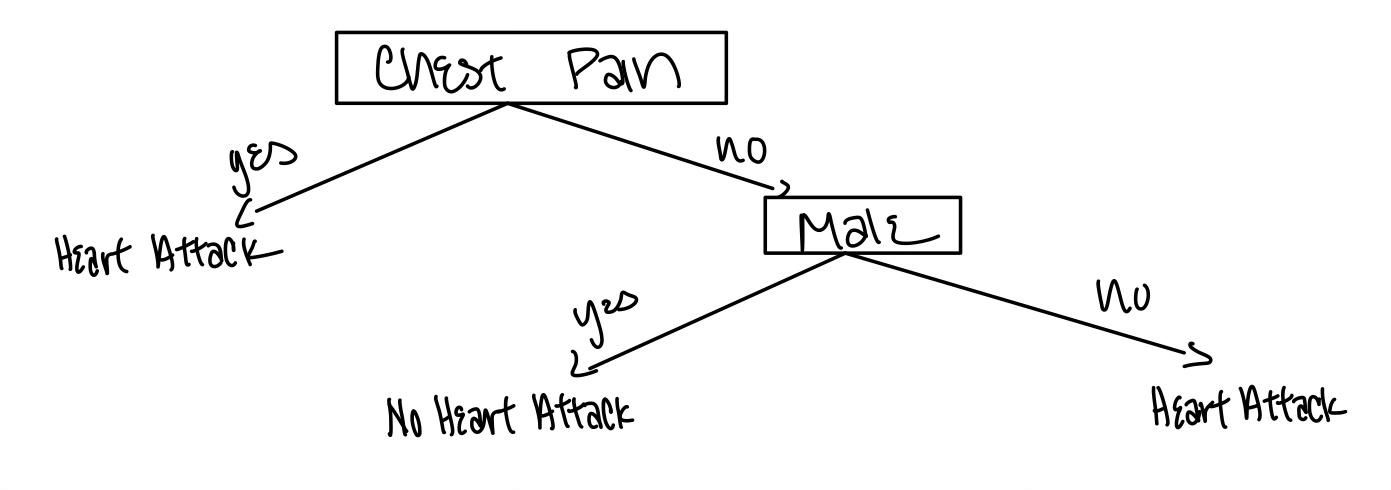
\includegraphics[scale=0.3]{./images/3.1_two}
\end{figure} \\

\subsection*{2.} If someone has chest pain, then we predict that they will have a heart attack. If they don't have chest pain, but they are male, then we predict that they will not have a heart attack. If they don't have chest pain but are female, then we predict that they will have a heart attack.


\newpage
\section{Backpropagation}
\subsection*{a)} We calculate the outputs at each level to get our final output.\\
$H_1 = (I_1)(W_{11}) + (I_2)(W_{21}) + 0.1 = (0.1)(1) + (0.2)(0.1) + 0.1 = 0.22$\\
$net_{H_1} = \frac{1}{1+e^{-H_1}} = \frac{1}{1+e^{-0.22}} = 0.555$\\\\
$H_2 = (I_1)(W_{12}) + (I_2)(W_{22}) + 0.1 = (0.1)(0.5) + (0.2)(0.2) + 0.1 = 0.19$\\
$net_{H_2} = \frac{1}{1+e^{-H_2}} = \frac{1}{1+e^{-0.19}} = 0.547$\\\\
$Output = (net_{H_1})(W_{13}) + (net_{H_2})(W_{23}) + 0.5 = (1)(0.555) + (0.5)(0.547) + 0.5 = 1.328$\\\\
$net_{Output} = \frac{1}{1+e^{-Output}} = \frac{1}{1+e^{-1.328}} = 0.791$\\\\
$Loss = -(ylog(\hat{y}) + (1-y)log(1-\hat{y}))$\\
$Loss = -(log(0.791)) = 0.235$\\

\subsection*{b)} $\frac{\partial{Loss}}{\partial{W_{11}}} = \frac{\partial{Loss}}{\partial{net_{Output}}} * \frac{\partial{net_{Output}}}{\partial{net_{H_1}}} * \frac{\partial{net_{H_1}}}{\partial{W_{11}}}$\\
$Loss = -(ylog(\hat{y}) + (1-y)log(1-\hat{y}))$\\
$\frac{\partial{Loss}}{\partial{net_{Output}}} = -(\frac{y}{\hat{y}} - \frac{1-y}{1-\hat{y}})$\\
$\frac{\partial{Loss}}{\partial{net_{Output}}} = -\frac{1}{0.791} = -1.264$\\\\
$net_{Output} = \frac{1}{1+e^{(net_{H_1})(W_{13}) + (net_{H_2})(W_{23}) + 0.5}}$\\
$net_{Output} = (1+e^{(net_{H_1})(W_{13}) + (net_{H_2})(W_{23}) + 0.5})^{-1}$\\
$\frac{\partial{net_{Output}}}{\partial{net_{H_1}}} = -(1+e^{(net_{H_1})(W_{13}) + (net_{H_2})(W_{23}) + 0.5})^{-2}(-W_{13}e^{-((W_{13})(net_{H_1})+(W_{23})(net_{H_2})+0.5)})$\\
$\frac{\partial{net_{Output}}}{\partial{net_{H_1}}} = 0.1656$\\\\
$net_{H_1} = \frac{1}{1+e^{(I_1)(W_{11}) + (I_2)(W_{21}) + 0.1}}$\\
$net_{H_1} = (1+e^{(I_1)(W_{11}) + (I_2)(W_{21}) + 0.1})^{-1}$\\
$\frac{\partial{H_1}}{\partial{W_{11}}} = -(1+e^{(I_1)(W_{11}) + (I_2)(W_{21}) + 0.1})^{-2}(-I_1e^{(I_1)(W_{11}) + (I_2)(W_{21}) + 0.1})$\\
$\frac{\partial{H_1}}{\partial{W_{11}}} = 0.0247$\\\\
$\frac{\partial{Loss}}{\partial{W_{11}}} = \frac{\partial{Loss}}{\partial{net_{Output}}} * \frac{\partial{net_{Output}}}{\partial{net_{H_1}}} * \frac{\partial{net_{H_1}}}{\partial{W_{11}}} = (-1.264)(0.1656)(0.0247) = -0.0052$

\subsection*{c)} $W_{11}' = W_{11} - \mu(\frac{\partial{Loss}}{\partial{W_{11}}})$\\
$W_{11}' = 1 - (0.1)(-0.0052)$\\
$W_{11}' = 1.00052$\\
$H_1' = (I_1)(W_{11}') + (I_2)(W_{21}) + 0.1$\\
$H_1' = (0.1)(1.00052) + (0.2)(0.1) + 0.1 = 0.22$\\
$net_{H_1}' = \frac{1}{1+e^{-H_1'}} = \frac{1}{1+e^{-0.22}} = 0.555$\\\\
$H_2' = (I_1)(W_{12}') + (I_2)(W_{22}) + 0.1$\\
$H_2' = (0.1)(0.5) + (0.2)(0.2) + 0.1 = 0.19$\\
$net_{H_2}' = \frac{1}{1+e^{-H_2'}} = \frac{1}{1+e^{-0.19}} = 0.547$\\\\
$Output' = (net_{H_1}')(W_{13}) + (net_{H_2}')(W_{23}) + 0.5 = (1)(0.555) + (0.5)(0.547) + 0.5 = 1.328$\\
$net_{Output} = \frac{1}{1+e^{-Output}} = \frac{1}{1+e^{-1.328}} = 0.7906$\\\\
$Loss = -(ylog(\hat{y}) + (1-y)log(1-\hat{y}))$\\
$Loss = -(log(0.7906)) = 0.235$\\
As we can see, the loss did not change by much.

\newpage
\section{Clustering}
\subsection*{a)} Since $\norm{\bar{x}_k-c_k} \leq d$, we know that after the first iteration, the center of the cluster won't move more than $d$, based on the equation that sets the new cluster center to $\frac{1}{N_j}\sum_{x_i\in C}^{x_i}$. Thus, since the cluster center can only move a certain amount, the clusters won't include any new points, and won't lose any of the data points. Thus, the centers will stop updating, and the algorithm converges after one iteration.

\subsection*{b)} If $d$ is alrge enough, re-clustering won't add or remove any data points from the cluster, so we will always converge after the first iteration.

\subsection*{c)} A clustering algorithm we can use that is more robust to outliers is DBSCAN, since it is density based. In the figure below, the left is an estimation of the clusters using K-means clustering, and the right is an estimation using DBSCAN. \\
\begin{figure}[h!]
  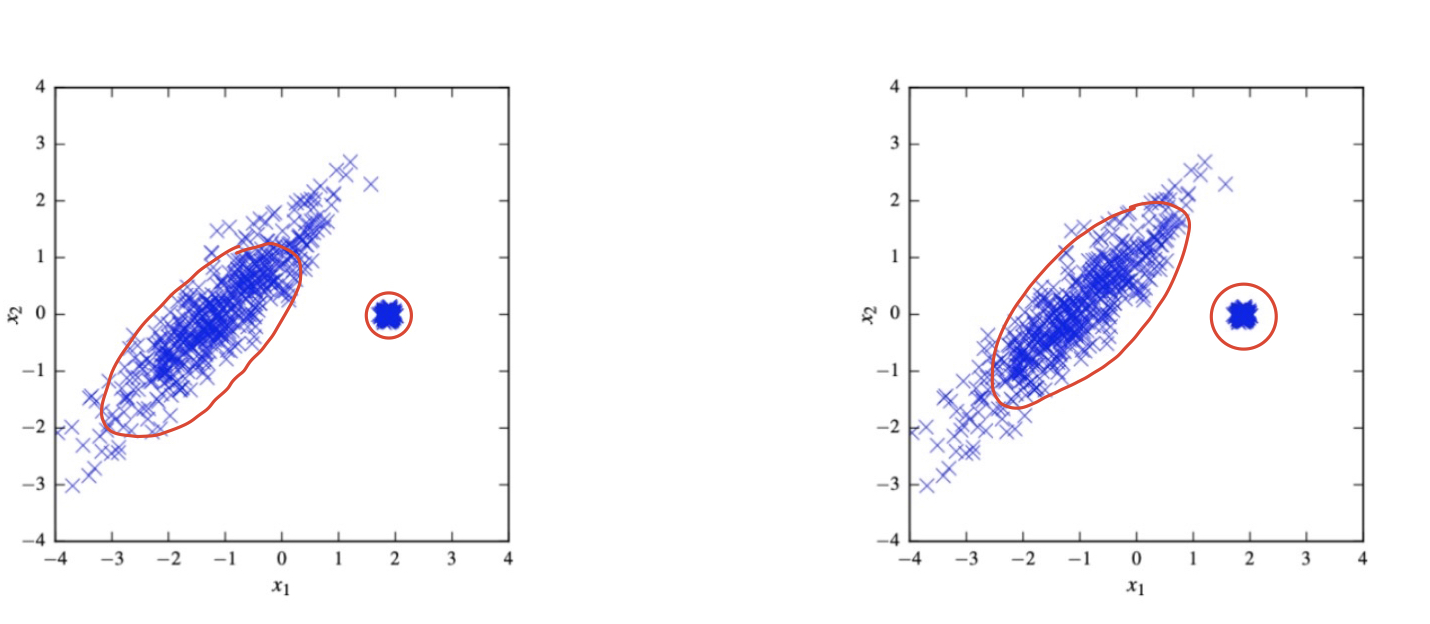
\includegraphics[scale=0.3]{./images/5c.jpeg}
\end{figure} \\
As we can see, using K-means pulls the center down, because of the outliers. In contrast, the plot of the right using DBSCAN has the clusters focused on areas where we have many points, so it is not as affected by outliers.


\newpage
\section{Decision Boundary}

\subsection*{(1)} The Linear SVM decision boundary corresponds to plot c, because it is a linear decision boundary that is equidistant from both classes.

\subsection*{(2)} Plot d likely corresponds to a polynomial kernel of degree 2, because the boundary resembles a polynomal graph.

\subsection*{(3)} The Perceptron decision boundary corresponds to plot b, because this is another linear plot, but it has a slope not equal to zero, so it's not the linear or logistic boundary.

\subsection*{(4)} The Logistic Regression boundary corresponds to plot a, because this is also a lineary boundary, but since there are more red points that blue, it'll try to maximize the distance from the red points.

\subsection*{(5)} Plot g corresponds to a decsion tree, because the boundary is very precise and overfitted to the data.

\subsection*{(6)} Plot h corresponds to a random forest, because it produces a similar boundary as a decision tree, but since it takes random samples of data, it is more generalized.

\subsection*{(7)} Plot f corresponds to a neural network with 1 hidden layer with 10 ReLU. This is because of its "rough" edges.

\subsection*{(8)} Plot e corresponds to a neural network with 1 hidden layer with 10 tanh units. This is because it's very similar to the other neural network, but since it's a smoother function, it likely uses tanh units.


\end{document}